\section{Feedforward MLP}
\subsection{Navigating through the indices}

\begin{frame}\frametitle{MLP}

\mode<article>{
The nodes in a feedforward neural network form a directed acyclic graph (DAG). There are no connections that feed back to a neuron in an earlier layer. A neuron can only be connected to another neuron that lies in a deeper layer in the network. We will eventually cover neural architectures that allow for feedback connections such as recurrent neural networks.
\figref{fig:mlp_arch} is an example MLP architecture (simplified by omitting bias nodes).
}

\begin{figure}[ht]
    \centering
	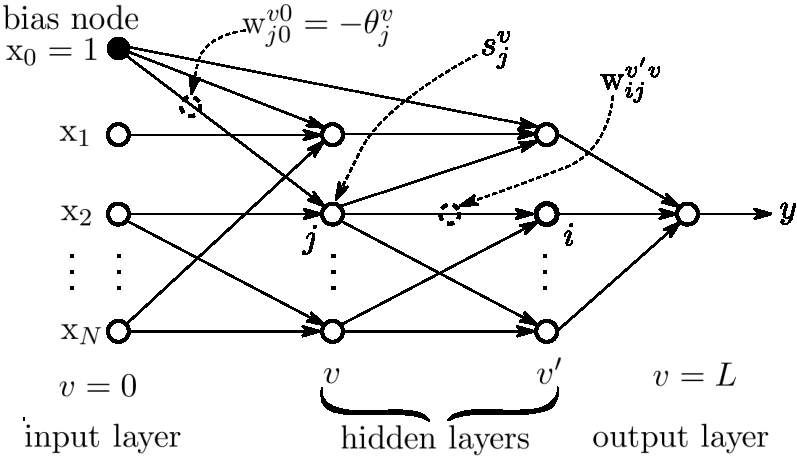
\includegraphics[width=0.7\textwidth]{img/section1_fig14}
	\caption{MLP architecture}
	\label{fig:mlp_arch} 
\end{figure}

\mode<article>{
Each node in the network is a connectionist neuron. This implies that every individual neuron extracts some feature from the ``input'' it receives.
The ``input'' to a neuron can come from the observed data $\vec x$ or it could be the response of another neuron from an earlier layer in the network.
This also implies that \emph{for every neuron} their exists a hyperplane which is represented by some weights $\vec w$ and a bias $\theta$.

$s^v_j$ denotes the \emph{activity} of the neuron $j$-th in layer $v$, while $s^{v'}_i$ denotes the \emph{activity} of the neuron $i$-th in layer $v'$.
$h^v_j$ and $h^{v'}_i$ denotes the \emph{total input} for neuron $(v,j)$ and neuron $(v',i)$, respectively.
The activity $s^{v'}_i$ is obtained by applying a transfer function $f^{v'}_i(\cdot)$ to the total input $h^{v'}_i$ of neuron $(v',i)$:
}

\begin{equation}
s^{v'}_i = f^{v'}_i(h^{v'}_i)
\end{equation}

\mode<article>{
where common choices for $f^v_j(\cdot)$, depending on the layer, can be:
\begin{itemize}
\item the identity function: $f^v_j(h) := h$. Often for the input layer, i.e. $s^0_j = f^0_j(h^0_j) = f^0_j(x_j) = x_j$
\item logistic sigmoidal or $\tanh(h)$. Common for hidden neurons and output neurons (for classification tasks).
\end{itemize}

$v$ is a literal that is used to denote a specific layer in the network.\\
$v=0$ describes the \emph{input layer} which holds the observations $\vec x$.\\
$v=L$ describes the \emph{output layer} of the MLP. All the layers in between, if any, are referred to as \emph{hidden layers}. For example, the scalar output of an MLP can be referred to using:


\begin{equation}
y(\vec x;\vec w) = f^L_1(h^L_1)
\end{equation}

$v'$, $v''$ are used to describe layers relative to the current layer $v$. $v'=v+1$ and $v''=v'+1=v+2$ is a very common but this depends on how exactly any two nodes are connected. Therefore, talking about layers $v$, $v'$ and $v''$ needs to be put into the context of the connections between neurons. To elaborate:

$w_{ij}^{v'v}$ measures the strength of the connection \underline{from} $(v,j)$ \underline{to} $(v',i)$. Seeing $v'v$ in the superscript of the weight tells us that the two neurons are directly connected (1 hop).

$w_{j0}^{v0}$ measures the bias $-\theta_{j0}^{v0}$ for neuron $(v,j)$. 

}

\end{frame}

\definecolor{darkgreen}{rgb}{0,0.6,0}
\begin{frame}
\only<1>{\frametitle{MLP}
}
\only<2>{\frametitle{MLP with \textbf{fully connected} layers}
}

\mode<presentation>{
\begin{figure}[ht]
     \centering
     \savebox{\imagebox}{
     \only<1>{
	 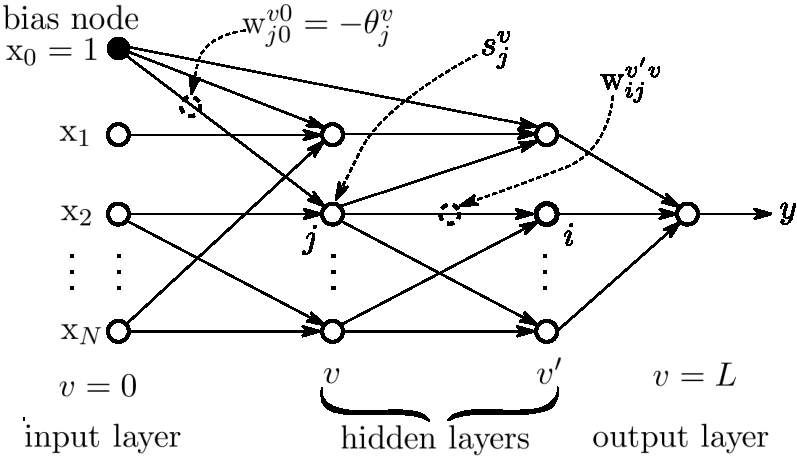
\includegraphics[width=0.4\textwidth]{img/section1_fig14}%
	 }
     \only<2->{
	 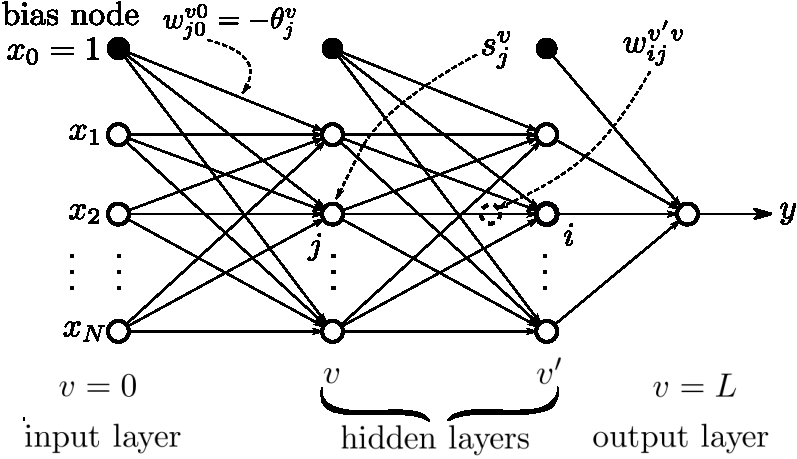
\includegraphics[width=0.4\textwidth]{img/section1_fig14_fc}%
	 }}%
     \begin{subfigure}[t]{0.5\textwidth}
         \centering
         \usebox{\imagebox}% Place largest image
     \end{subfigure}
     \hspace{10mm}
     \begin{subfigure}[t]{0.3\textwidth}
         \centering
         \raisebox{\dimexpr.5\ht\imagebox-.5\height}{% Raise smaller image into place
         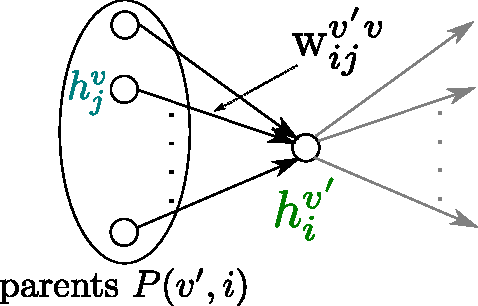
\includegraphics[width=0.9\textwidth]{img/section1_fig20_mini_vdi}
         }
     \end{subfigure}
\end{figure}
}

\mode<article>{

\begin{figure}
    \centering
	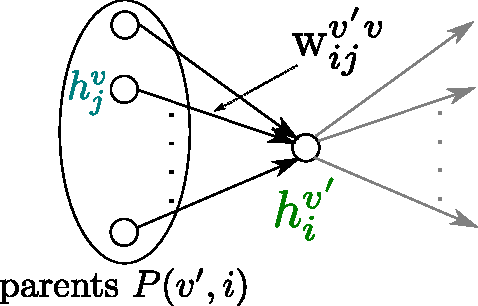
\includegraphics[width=0.33\textwidth]{img/section1_fig20_mini_vdi}
	\caption{Computing the total input for neuron $(v',i)$}
	\label{eq:compute_vdi}
\end{figure}
}

\mode<article>{
To formulate how neuron $(v', i)$ processes its input requires identifying the set of parent nodes $P(v', i)$ of neuron $(v',i)$. The weighted sum of the parent activations yields the total input ${\color{darkgreen}h^{v'}_i}$:
}
   
\only<-2>{
\begin{equation}
		{\color{darkgreen}h_i^{v'}} 
		:= 
		\kern-2ex
		\sum_{(\mu,k) \in P(v',\,i)}
		\kern-2ex
		w_{ik}^{v'\mu}\; 
		f_k^\mu\big( {\color{teal} h_k^\mu} \big)   
		\label{eq:total_input_vdi_pre},
\end{equation}
}

\mode<article>{
We now assume an architecture with \emph{fully connected layers}. This implies that every node in layer $v$ is connected to all nodes in the subsequent layer $v'$ (except for the bias node in $v'$ because it has no parents). This type of connectivity allows us to simplify the notation as it implies that the set of parents $P(v',\,i)$ is essentially a vector of all activations in layer $v$:
}

\only<2>{
\slidesonly{
Full connectivity implies
}
\begin{equation}
P(v',i) := (
\underbrace{
s^v_0}_{\substack{=1\\ \text{(bias)}}
}
, s^v_1, \ldots, s^v_j, \ldots, s^v_{N_v})^\top,
\end{equation}

where $N_v$ is the number of hidden nodes in layer $v$. 

\notesonly{From this follows:}
}

\only<3>{

\begin{align}
		{\color{darkgreen}h_i^{v'}} 
		:=& 
		\kern-2ex
		\sum_{(\mu,k) \in P(v',\,i)}
		\kern-2ex
		w_{ik}^{v'\mu}\; 
		f_k^\mu\big( {\color{teal} h_k^\mu} \big) \\
		{\color{darkgreen}h_i^{v'}} \;
		\stackrel{\mathclap{
\substack{\text{\tiny fully}\\\text{\tiny conn.}}}
}{=}& 
		\kern1.5ex
		\sum_{j=0}^{N_v}
		w_{ij}^{v'v}\; 
		f_j^v\big( {\color{teal} h_j^v} \big)\\
		=& 
		\kern1.5ex
		{\vec w_{i}^{v'v}}^\top
		\kern-1ex
		\cdot  
		\vec f^v\big( {\color{teal} \vec h^v} \big)\\
		=& 
		\kern1.5ex
		{\vec w_{i}^{v'v}}^\top
		\kern-1ex
		\cdot
		\vec s^v\\
\end{align}

\slidesonly{\vspace{-5mm}}
here $\vec w_{i}^{v'v} := \big(
\underbrace{
w_{i0}^{v'v}}_{\text{bias}}
, w_{i1}^{v'v}, \ldots,w_{iN_v}^{v'v}\big)^\top \in \R^{N_v+1}$
}

\only<4>{
\notesonly{
Consequently, to compute} the total input for all $N_{v'}$ neurons in the layer $v$\notesonly{ we introduce the weight matrix 
$\vec W^{v'v} := \big({\vec w_1^{v'v}}^\top, {\vec w_2^{v'v}}^\top, \ldots, {\vec w_{N_{v'}}^{v'v}}^\top\big)$:}
\begin{equation}
\vec W^{v'v} = 
\left(
\begin{array}{cccccc}
\Big| & \Big| & & \Big| & & \Big| \\[3mm]
\vec w_{1}^{v'v} & \vec w_{2}^{v'v} & \cdots & \vec w_{i}^{v'v} & \cdots & \vec w_{N_{v'}}^{v'v}\\[2mm]
\Big| & \Big| & & \Big| & & \Big|
\end{array}
\right) \in \R^{(N_v+1) \times N_{v'}}
\end{equation}

Therefore,

\begin{equation}
		{\color{darkgreen} \vec h^{v'}} 
		=
		{\vec W^{v'v}}^\top
		\kern-1ex
		\cdot
		\vec f^v\big( {\color{teal} \vec h^v} \big)
		=
		\kern1.5ex
		{\vec W^{v'v}}^\top
		\kern-1ex
		\cdot
		\vec s^v
\end{equation}
}

\end{frame}
